\documentclass[11pt]{article}
\usepackage[utf8]{inputenc}


\usepackage{url}
\usepackage{breakurl}
\usepackage[breaklinks]{hyperref}
\usepackage[super]{nth}
\usepackage{bm}
\usepackage{booktabs}
\usepackage{enumerate}
\usepackage{graphicx}
\usepackage{multirow}
\usepackage{multicol}
\usepackage{amsmath}
\usepackage{amstext}
\usepackage{amssymb}
\usepackage{pdflscape}
\usepackage{multirow}
\usepackage{amsfonts}
\usepackage{rotating}
\usepackage{xcolor}
\usepackage{placeins}
\usepackage{amssymb,algorithm,algorithmic,algpseudocode}
\usepackage{natbib}
\usepackage{setspace} 
\usepackage{latexsym}
\usepackage{subfig}
\allowdisplaybreaks
\usepackage{array}
\usepackage{subcaption}
\newcolumntype{H}{>{\setbox0=\hbox\bgroup}c<{\egroup}@{}}
\usepackage{pdfpages}
\usepackage{diagbox}
\usepackage{graphicx}
\usepackage{soul}

\usepackage{capt-of}% or \usepackage{caption}
\usepackage{varwidth}
\newsavebox\tmpbox

\usepackage{csvsimple,booktabs}
\usepackage{filecontents}

\usepackage{afterpage}
\graphicspath{{Images/}}


\usepackage{geometry}
\geometry{
	a4paper,
	total={160mm,220mm},
	%left=16mm,
	top=22mm,
	bottom=30mm,
}

\usepackage[linesnumbered,ruled,vlined]{algorithm2e}

\title{Campaign Optimization under Communication Limitations \\}
\author{Dursun Koc $^{a}$ \\ 
	e-mail: dursun.koc@turkcell.com.tr, \\\\
	Dilek Gunnec $^{a}$ \\ 
	e-mail: dilek.gunnec@ozyegin.edu.tr, ORCID ID: 0000-0002-0749-2584 \\\\
$^{a}$ Ozyegin University, Department of Industrial Engineering, Istanbul, Turkey \\ 
$^{\ast}$ Corresponding author \\ }
	
\date{}

\begin{document}
\maketitle
\begin{abstract}
The main objective for marketers is to introduce their companies’ products or services to their customers or potential customers. With this objective they have two different strategies; inbound and outbound marketing strategies. If a marketer wants to introduce a product with an outbound strategy she first selects a target audience, for example people living in a specific city, and age between 20 to 30 namely the young people, then she tries to send her message about the product to them with direct channels such as SMS, outbound call-center or IVR calls. On the other hand, if she wants to introduce her product with an inbound strategy, first she decides rules of whom to interact with. When a customer visits any of the inbound channels for example a web-page or inbound call-center, and the customer fulfills the rules, the message is given to the customer. So inbound marketing is also considered as content marketing. The marketer creates content and tries to gain interests of the customer using social media tactics whereas outbound marketing strategy depends on mass media tools to push the message about the product or the service. Outbound marketing is mostly seen as interruptive and the target audience can easily find a way to dismiss the message. \\

Keywords: Campaign Optimization, Knapsack Problem, Greedy Heuristic, Multi-dimensional Knapsack Problem.

\end{abstract}


\newpage

\section{Introduction}

The main objective for marketers is to introduce their companies’ products or services to their customers or potential customers. With this objective they have two different strategies; inbound and outbound marketing strategies. If a marketer wants to introduce a product with an outbound strategy she first selects a target audience, for example people living in a specific city, and age between 20 to 30 namely the young people, then she tries to send her message about the product to them with direct channels such as SMS, outbound call-center or IVR calls. On the other hand, if she wants to introduce her product with an inbound strategy, first she decides rules of whom to interact with. When a customer visits any of the inbound channels for example a web-page or inbound call-center, and the customer fulfills the rules, the message is given to the customer. So inbound marketing is also considered as content marketing. The marketer creates content and tries to gain interests of the customer using social media tactics whereas outbound marketing strategy depends on mass media tools to push the message about the product or the service. Outbound marketing is mostly seen as interruptive and the target audience can easily find a way to dismiss the message. Besides, from the companies’ perspective it can be very inefficient; because sending a message to a customer who is unlikely to respond is a cost; moreover, not sending the message to a customer who is more likely to respond is a loss from revenue \citep{sarkar}. Deciding who should receive a specific offer is one of the essential questions of outbound (direct) marketing. Marketers have to wisely identify the right target audience because the key to a good relationship with customers is keeping your offers relevant to the customers’ need \citep{malthouse}. An irrelevant communication with customer can cause irritation, and they can block the communication channel, so the company will lose its chance to make a relevant or profitable communication opportunity in the future. Finding the right target audience will not make outbound marketing communication perfect, the most appropriate communication channel and the right time should also be found, and any opportunity to connect to the customers in the future should not be lost.\\

Outbound marketing (also called targeted advertising) needs large amount of personal data of customers, for being effective. So companies are collecting more information about their customers, which causes an information asymmetry \citep{waerdt}. As the governments are responsible for protecting their citizens’ rights, they make laws and regulations on this information asymmetry. The General Data Protection Regulation (GDPR) law in EU is an example. According to such regulations; a customer can request from the company to stop processing its data. Therefore, companies need to apply some limitation on outbound communication to their companies.\\

Outbound marketing campaigns need to be very well planned and optimized with regard to time, target audience, channel and content. In this study we will optimize outbound campaigns regarding time and channel with keeping communication under certain limitations, those limitations can either be a result of legislation or a result of marketing strategy not to irritate customer.\\

The remaining of this paper is structured as follows. In \S \ref{s:literature-review}, we review the related literature. In \S \ref{s:problem-model}, we describe the problem and present our mathematical model. In \S \ref{s:solution-method}, we describe our solution methods. In \S \ref{num-analysis}, we present computational results. Finally, we present our conclusions in \S \ref{s:conclusion}.


%%%%%%%%%%%%%%%%%%%%%%%%%%%%%%%%%%%%%%%%%%%%%%%%%%%%%%%%%%
%%%%%%%%%%%%%%%%%%%%%%%%%%%%%%%%%%%%%%%%%%%%%%%%%%%%%%%%%%


\section{Literature Review}  \label{s:literature-review}

In the industry, outbound campaigns are mostly designed regarding the target audience. Machine learning methods, statistics and business rules and regulations are used to find the right target audience, and the message about the product is sent to customers; moreover database marketing community also tries to estimate the expected value of an offer to a specific customer from a specific channel \citep{cohen_exp, oliveira_hypr}. In direct marketing, marketers select a portion of the customer group with the highest probability of expecting the offer, and then add them to their target audience for the marketing campaign \citep{owczarczuk}. However, even if the offer addresses the customer’s need, most of the time customer can dismiss the message because of the wrong channel or because of the wrong time. Having the right channel and the right time with the right audience is the most desired case, but it is not free. The cost of some channels can be high while some others are cheaper. Further, with social network effects some of the targeting can become unnecessary and costly.\\

In today’s world, marketers have multiple channels to introduce their product or services, and many studies have shown the importance of omni-channel sales strategies \citep{shankar, park}. In the essence customers want to interact with the company via multiple channels, companies’ challenge is to provide a nearly identical environment for each channel \citep{bell}. Customer can get information about a product or service from one channel, but the purchase can be from another channel \citep{park}. Even the information about the product or service can be solidified by a series of messages from different channels. At this point it is crucial to employ additional constraints regarding multiple channels when optimizing the campaign.\\

Most of the studies about campaign optimization focus on obtaining the right target audience for the campaign \citep{goul}; however, they usually ignore campaign channels, or optimize the online campaigns. They are finding the best matched campaign for a given online search only, or web-page banner optimization \citep{liu}, and the success criteria or the objective function for such models is often the click through rate or the action rate. Such objective functions do not truly represent the advertisers’ benefit and rather focus on the publishers’ benefit \citep{altshuler}. Our model will be directly related to the advertisers’ benefit.\\

Different studies work on different industries and various business constraints; but the mathematical models mostly seems similar, and can be counted as assignment problem, or more specifically multi-dimensional knapsack problem \citep{cohen_exp, oliveira_hypr}. For solving ILP (Integer Linear Programming), MIP(Mixed Integer Programming) models, numerous methods and tools have been introduced\citep{fallah_bb, chu_mip}, however due to the complexity of the problem, handling big models remains a technical difficulty. Although the branch and bound (B&B) algorithm has been presented as the definitive and deterministic solution, when the number of variables and the number of constraints get larger, the B&B algorithm does not provide a solution in reasonable time \citep{herrera_pbb, sato}. Because of that reason some work on parallel B&B algorithm\citep{fallah_bb, sato}; but computational resources required to run the algorithm increases.\\ \citeauthor{cohen_exp} applied a greedy approach to a similar problem \citep{cohen_exp}. Multidimensional knapsack problems having multiple resource constraints with binary decision variables, which is similar to our model have been dealt with greedy-like heuristic methods \citep{akcay_mdkp}.

Although studies related to campaign management are common in marketing, there is increasing interest to this area from operations research and computer science areas, as the abundant data require complex data analysis skills. In my thesis, after such data analysis, we plan to introduce optimization methods which are not yet commonly used to tackle such problems. Specifically, one of our main contributions will be utilizing from network optimization tools to produce high quality solutions.\\

In this study, we plan to develop a model which tries to maximize the number of interactions for the campaigns decided by marketing team, while not exceeding the communication limitations. In the second place, we also try to increase the number of interaction to the most influential customers. We believe that influential customers can spread our message to a broader audience. In order to find the influential customer we will use customers' call and product purchase data from Turkcell.

\section{Problem Definition and Mathematical Model}  \label{s:problem-model}

In this section, we describe the proposed mathematical model to maximize the number of interactions to customer by adhering the communication limitations. In \S \ref{s:problem-desc}, we detail the limitations to customer communication and in \S \ref{s:problem-math}, we present our mathematical model.

\subsection{Problem Description} \label{s:problem-desc}

Turkcell, a telecommunication company in Turkey, provides different tariffs, services and product to its customers. In order to introduce these services and products to its customers and potential customers, the marketing team launches daily and weekly basis campaigns. Before launching these campaigns, they do some data analysis to find the right targeting group. After finding the right target audience, they apply a set of business rules to optimize their communication with their customers. During this optimization process, filters are applied to the target audience in order to keep the communication to customers in certain levels. The first filter assure that no customers are targeted by the same campaign from different channels. Next, they limit the number of total interactions to a customer in one day. Campaigns are categorized in two dimensions; first dimension is quota categories which describes filters for a campaign and the second one is priority categories which describes the importance of a campaign. Each campaign belongs to a quota category and each quota category has a limitation on the number of messages sent to a customer, both in a daily, and a weekly basis; moreover each campaign has a limitation unique to its own; and finally, each communication channel has a capacity that should not be exceeded for each day. Each campaign is bound to a priority category.\\

Turkcell launches about 70 campaigns on average for around 60-70 million customers through 3 channels each day, and these campaigns are planned in a weekly basis. Number of quota categories is fixed to 3, but priority categories can be variable around 10.\\

In our study to optimize the Turkcell’s outbound campaign management we start with an initial model that accepts the target audience without any inference, but in the next steps we will shrink the target audience using network optimization technics. The motivation behind using network optimization is the idea that people communicating can carry our message.

\subsection{Mathematical Model} \label{s:problem-math}

In this section, we present a mixed integer programming model for the campaign optimization problem described at \S \ref{s:problem-desc}. We first introduce the notation and then present the mathematical model.\\

% General Math Model
\noindent \textbf{Sets}\\

\noindent ${\mathcal{C}}$: set of campaigns. \\
\noindent ${\mathcal{U}}$: set of customers. \\
\noindent ${\mathcal{H}}$: set of channels. \\
\noindent ${\mathcal{D}}$: set of planning days. \\
\noindent ${\mathcal{I}}$: set of quota categories. \\
\noindent ${\mathcal{P}}$: set of priority categories. \\


\noindent \textbf{Decision Variables}\\

\noindent $X_{{c}{u}{h}{d}}=1$, if campaign $c \in \mathcal{C}$ will be sent to customer $u \in \mathcal{U}$ through channel $h \in \mathcal{H}$ at day $d \in \mathcal{D}$, and 0 otherwise.
($\forall c \in \mathcal{C}$, $\forall u \in \mathcal{U}$, $\forall h \in \mathcal{H}$, $\forall d \in \mathcal{D}$ )\\

\noindent \textbf{Parameters}\\

\noindent $e_{{c}{u}}=1$, if customer $u \in \mathcal{U}$ is eligible for campaign $c \in \mathcal{C}$, and 0 otherwise.
($\forall c \in \mathcal{C}$, $\forall u \in \mathcal{U}$)\\

\noindent $s_{{c}{u}{h}{d}}=1$, if customer $u \in \mathcal{U}$ received a communication for campaign $c \in \mathcal{C}$, through channel $h \in \mathcal{H}$, at day $d \in \mathcal{D}$ previous week and 0 otherwise.
($\forall c \in \mathcal{C}$, $\forall u \in \mathcal{U}$, $\forall h \in \mathcal{H}$, $\forall d \in \mathcal{D}$ )\\

\noindent $q_{{i}{c}}=1$, if campaign $c \in \mathcal{C}$ is in $i \in \mathcal{I}$ quota category, and 0 otherwise.
($\forall c \in \mathcal{C}$, $\forall i \in \mathcal{I}$)\\

\noindent $r_{{c}{p}}$ priority value of campaign $c \in \mathcal{C}$ regarding priority type $p \in \mathcal{P}$.
($\forall c \in \mathcal{C}$, $\forall p \in \mathcal{P}$)\\

\noindent $b$ communication limit per customer $u \in \mathcal{U}$ for the whole period.
($\forall u \in \mathcal{U}$)\\

\noindent $k$ communication limit per customer $u \in \mathcal{U}$ at each day.
($\forall u \in \mathcal{U}$)\\

\noindent $l_{c}$ communication limit per customer $u \in \mathcal{U}$ for campaign $c \in \mathcal{C}$.
($\forall c \in \mathcal{C}$, $\forall u \in \mathcal{U}$)\\

\noindent $m_{i}$ communication limit per customer $u \in \mathcal{U}$ for $i \in \mathcal{I}$ quota category for the whole period.
($\forall u \in \mathcal{U}$, $\forall i \in \mathcal{I}$)\\

\noindent $n_{i}$ communication limit per customer $u \in \mathcal{U}$ for $i \in \mathcal{I}$ quota category at each day.
($\forall d \in \mathcal{D}$, $\forall u \in \mathcal{U}$, $\forall i \in \mathcal{I}$)\\

\noindent $t_{{h}{d}}$ capacity for channel $h \in \mathcal{H}$ at day $d \in \mathcal{D}$.
($\forall h \in \mathcal{H}$, $\forall d \in \mathcal{D}$)\\

\noindent The formulation for the campaign optimization is presented next.

\begin{align}
\text{Maximize} & \displaystyle
\sum\limits_{p\in \mathcal{P}}
\sum\limits_{c\in \mathcal{C}}
\sum\limits_{u\in \mathcal{U}}
\sum\limits_{h\in \mathcal{H}}
\sum\limits_{d\in \mathcal{D}}
X_{{c}{u}{h}{d}} \cdot r_{{c}{p}} \label{mathmodel_obj}&
\\
\text{subject to} \notag\\
&X_{{c}{u}{h}{d}} \leq e_{{c}{u}},&\forall c \in \mathcal{C}, \forall u \in \mathcal{U}, \forall h \in \mathcal{H}, \forall d \in \mathcal{D} \label{mathmodel_eligibility}&\\
&\sum\limits_{h\in\mathcal{H}}X_{{c}{u}{h}{d}} \leq 1, &\forall c \in \mathcal{C}, \forall u \in \mathcal{U}, \forall d \in \mathcal{D} \label{mathmodel_singlechannel}&\\
&\sum\limits_{h\in\mathcal{H}}\sum\limits_{c\in\mathcal{C}}\sum\limits_{d\in\mathcal{D}}X_{{c}{u}{h}{d}} \leq b, &\forall u \in \mathcal{U} \label{mathmodel_percustomercommlimit}&\\
&\sum\limits_{h\in\mathcal{H}}\sum\limits_{c\in\mathcal{C}}\sum\limits_{d\in [1]}X_{{c}{u}{h}{d}} + \sum\limits_{h\in\mathcal{H}}\sum\limits_{c\in\mathcal{C}}\sum\limits_{d\in [2,7]}s_{{c}{u}{h}{d}} \leq b, &\forall u \in \mathcal{U} \label{mathmodel_percustomercommlimit_rh1}&\\
&\sum\limits_{h\in\mathcal{H}}\sum\limits_{c\in\mathcal{C}}\sum\limits_{d\in [1,2]}X_{{c}{u}{h}{d}} + \sum\limits_{h\in\mathcal{H}}\sum\limits_{c\in\mathcal{C}}\sum\limits_{d\in [3,7]}s_{{c}{u}{h}{d}} \leq b, &\forall u \in \mathcal{U} \label{mathmodel_percustomercommlimit_rh2}&\\
&\sum\limits_{h\in\mathcal{H}}\sum\limits_{c\in\mathcal{C}}\sum\limits_{d\in [1,3]}X_{{c}{u}{h}{d}} + \sum\limits_{h\in\mathcal{H}}\sum\limits_{c\in\mathcal{C}}\sum\limits_{d\in [4,7]}s_{{c}{u}{h}{d}} \leq b, &\forall u \in \mathcal{U} \label{mathmodel_percustomercommlimit_rh3}&\\
&\sum\limits_{h\in\mathcal{H}}\sum\limits_{c\in\mathcal{C}}\sum\limits_{d\in [1,4]}X_{{c}{u}{h}{d}} + \sum\limits_{h\in\mathcal{H}}\sum\limits_{c\in\mathcal{C}}\sum\limits_{d\in [5,7]}s_{{c}{u}{h}{d}} \leq b, &\forall u \in \mathcal{U} \label{mathmodel_percustomercommlimit_rh4}&\\
&\sum\limits_{h\in\mathcal{H}}\sum\limits_{c\in\mathcal{C}}\sum\limits_{d\in [1,5]}X_{{c}{u}{h}{d}} + \sum\limits_{h\in\mathcal{H}}\sum\limits_{c\in\mathcal{C}}\sum\limits_{d\in [6,7]}s_{{c}{u}{h}{d}} \leq b, &\forall u \in \mathcal{U} \label{mathmodel_percustomercommlimit_rh5}&\\
&\sum\limits_{h\in\mathcal{H}}\sum\limits_{c\in\mathcal{C}}\sum\limits_{d\in [1,6]}X_{{c}{u}{h}{d}} + \sum\limits_{h\in\mathcal{H}}\sum\limits_{c\in\mathcal{C}}\sum\limits_{d\in [7]}s_{{c}{u}{h}{d}} \leq b, &\forall u \in \mathcal{U} \label{mathmodel_percustomercommlimit_rh6}&\\
&\sum\limits_{h\in\mathcal{H}}\sum\limits_{c\in\mathcal{C}}X_{{c}{u}{h}{d}} \leq k, &\forall u \in \mathcal{U}, \forall d \in \mathcal{D} \label{mathmodel_percustomercommlimit_day}&\\
&\sum\limits_{d\in\mathcal{D}}\sum\limits_{h\in\mathcal{H}}X_{{c}{u}{h}{d}} \leq l_{c}, &\forall c \in \mathcal{C}, \forall u \in \mathcal{U} \label{mathmodel_percustomercamplimit}&\\
&\sum\limits_{d\in[1]}\sum\limits_{h\in\mathcal{H}}X_{{c}{u}{h}{d}} + \sum\limits_{d\in[2,7]}\sum\limits_{h\in\mathcal{H}}s_{{c}{u}{h}{d}} \leq l_{c}, &\forall c \in \mathcal{C}, \forall u \in \mathcal{U} \label{mathmodel_percustomercamplimit_rh1}&\\
&\sum\limits_{d\in[1,2]}\sum\limits_{h\in\mathcal{H}}X_{{c}{u}{h}{d}} + \sum\limits_{d\in[3,7]}\sum\limits_{h\in\mathcal{H}}s_{{c}{u}{h}{d}} \leq l_{c}, &\forall c \in \mathcal{C}, \forall u \in \mathcal{U} \label{mathmodel_percustomercamplimit_rh2}&\\
&\sum\limits_{d\in[1,3]}\sum\limits_{h\in\mathcal{H}}X_{{c}{u}{h}{d}} + \sum\limits_{d\in[4,7]}\sum\limits_{h\in\mathcal{H}}s_{{c}{u}{h}{d}} \leq l_{c}, &\forall c \in \mathcal{C}, \forall u \in \mathcal{U} \label{mathmodel_percustomercamplimit_rh3}&\\
&\sum\limits_{d\in[1,4]}\sum\limits_{h\in\mathcal{H}}X_{{c}{u}{h}{d}} + \sum\limits_{d\in[5,7]}\sum\limits_{h\in\mathcal{H}}s_{{c}{u}{h}{d}} \leq l_{c}, &\forall c \in \mathcal{C}, \forall u \in \mathcal{U} \label{mathmodel_percustomercamplimit_rh4}&\\
&\sum\limits_{d\in[1,5]}\sum\limits_{h\in\mathcal{H}}X_{{c}{u}{h}{d}} + \sum\limits_{d\in[6,7]}\sum\limits_{h\in\mathcal{H}}s_{{c}{u}{h}{d}} \leq l_{c}, &\forall c \in \mathcal{C}, \forall u \in \mathcal{U} \label{mathmodel_percustomercamplimit_rh5}&\\
&\sum\limits_{d\in[1,6]}\sum\limits_{h\in\mathcal{H}}X_{{c}{u}{h}{d}} + \sum\limits_{d\in[7]}\sum\limits_{h\in\mathcal{H}}s_{{c}{u}{h}{d}} \leq l_{c}, &\forall c \in \mathcal{C}, \forall u \in \mathcal{U} \label{mathmodel_percustomercamplimit_rh6}&\\
&\sum\limits_{d\in\mathcal{D}}\sum\limits_{h\in\mathcal{H}}\sum\limits_{c\in\mathcal{C}}X_{{c}{u}{h}{d}} \cdot q_{{i}{c}} \leq m_{i}, &\forall u \in \mathcal{U}, \forall i \in \mathcal{I} \label{mathmodel_weeklyquotalimit}&\\
&\sum\limits_{d\in[1]}\sum\limits_{h\in\mathcal{H}}\sum\limits_{c\in\mathcal{C}}X_{{c}{u}{h}{d}} \cdot q_{{i}{c}} + \sum\limits_{d\in[2,7]}\sum\limits_{h\in\mathcal{H}}\sum\limits_{c\in\mathcal{C}}s_{{c}{u}{h}{d}} \cdot q_{{i}{c}} \leq m_{i}, &\forall u \in \mathcal{U}, \forall i \in \mathcal{I} \label{mathmodel_weeklyquotalimit_rh1}&\\
&\sum\limits_{d\in[1,2]}\sum\limits_{h\in\mathcal{H}}\sum\limits_{c\in\mathcal{C}}X_{{c}{u}{h}{d}} \cdot q_{{i}{c}} + \sum\limits_{d\in[3,7]}\sum\limits_{h\in\mathcal{H}}\sum\limits_{c\in\mathcal{C}}s_{{c}{u}{h}{d}} \cdot q_{{i}{c}} \leq m_{i}, &\forall u \in \mathcal{U}, \forall i \in \mathcal{I} \label{mathmodel_weeklyquotalimit_rh2}&\\
&\sum\limits_{d\in[1,3]}\sum\limits_{h\in\mathcal{H}}\sum\limits_{c\in\mathcal{C}}X_{{c}{u}{h}{d}} \cdot q_{{i}{c}} + \sum\limits_{d\in[4,7]}\sum\limits_{h\in\mathcal{H}}\sum\limits_{c\in\mathcal{C}}s_{{c}{u}{h}{d}} \cdot q_{{i}{c}} \leq m_{i}, &\forall u \in \mathcal{U}, \forall i \in \mathcal{I} \label{mathmodel_weeklyquotalimit_rh3}&\\
&\sum\limits_{d\in[1,4]}\sum\limits_{h\in\mathcal{H}}\sum\limits_{c\in\mathcal{C}}X_{{c}{u}{h}{d}} \cdot q_{{i}{c}} + \sum\limits_{d\in[5,7]}\sum\limits_{h\in\mathcal{H}}\sum\limits_{c\in\mathcal{C}}s_{{c}{u}{h}{d}} \cdot q_{{i}{c}} \leq m_{i}, &\forall u \in \mathcal{U}, \forall i \in \mathcal{I} \label{mathmodel_weeklyquotalimit_rh4}&\\
&\sum\limits_{d\in[1,5]}\sum\limits_{h\in\mathcal{H}}\sum\limits_{c\in\mathcal{C}}X_{{c}{u}{h}{d}} \cdot q_{{i}{c}} + \sum\limits_{d\in[6,7]}\sum\limits_{h\in\mathcal{H}}\sum\limits_{c\in\mathcal{C}}s_{{c}{u}{h}{d}} \cdot q_{{i}{c}} \leq m_{i}, &\forall u \in \mathcal{U}, \forall i \in \mathcal{I} \label{mathmodel_weeklyquotalimit_rh5}&\\
&\sum\limits_{d\in[1,6]}\sum\limits_{h\in\mathcal{H}}\sum\limits_{c\in\mathcal{C}}X_{{c}{u}{h}{d}} \cdot q_{{i}{c}} + \sum\limits_{d\in[7]}\sum\limits_{h\in\mathcal{H}}\sum\limits_{c\in\mathcal{C}}s_{{c}{u}{h}{d}} \cdot q_{{i}{c}} \leq m_{i}, &\forall u \in \mathcal{U}, \forall i \in \mathcal{I} \label{mathmodel_weeklyquotalimit_rh6}&\\
&\sum\limits_{h\in\mathcal{H}}\sum\limits_{c\in\mathcal{C}}X_{{c}{u}{h}{d}} \cdot q_{{i}{c}} \leq n_{i}, &\forall u \in \mathcal{U}, \forall d \in \mathcal{D}, \forall i \in \mathcal{I} \label{mathmodel_dailyquotalimit}&\\
&\sum\limits_{u\in\mathcal{U}}\sum\limits_{c\in\mathcal{C}}X_{{c}{u}{h}{d}} \leq t_{{h}{d}}, &\forall d \in \mathcal{D}, \forall h \in \mathcal{H} \label{mathmodel_channellimit}&\\
&X_{{c}{u}{h}{d}} \in \{0,1\},&\forall c \in \mathcal{C}, \forall u \in \mathcal{U}, \forall h \in \mathcal{H}, \forall d \in \mathcal{D} \label{mathmodel_integrity}
\end{align}\\

The objective function \eqref{mathmodel_obj} maximizes campaign communication regarding the campaign priority. Constraints \eqref{mathmodel_eligibility} ensure that the communication will be placed when the customer is eligible for the campaign. Constraints \eqref{mathmodel_singlechannel} say that a customer should not be targeted for the same campaign from different channels. Constraints \eqref{mathmodel_percustomercommlimit} defines an upper-bound for total number of communication to each customer for the whole period; and constraints from \eqref{mathmodel_percustomercommlimit_rh1} to \eqref{mathmodel_percustomercommlimit_rh6} extends the upper-bound for total number of communication to each customer regarding the previous period. Constraints \eqref{mathmodel_percustomercommlimit_day} defines an upper-bound for total number of communication to each customer for a single day. Constraints \eqref{mathmodel_percustomercamplimit} defines an upper-bound for total number of communication to each customer per campaign for the whole period; and constraints from \eqref{mathmodel_percustomercamplimit_rh1} to \eqref{mathmodel_percustomercamplimit_rh6} extends the upper-bound for total number of communication to each customer per campaign regarding the previous period. Campaigns are group by their marketing purpose, and for each of these groups we have combined limitations, constraints \eqref{mathmodel_weeklyquotalimit} draws a limitation on the number of communications about campaigns that fell in specific groups. $q_{{i}{c}}$ stands for if the campaign $c$ is in the $i$ category. Likewise constraints from \eqref{mathmodel_weeklyquotalimit_rh1} to \eqref{mathmodel_weeklyquotalimit_rh6} limits the number of communications for campaign quota categories regarding previous period. Constraints \eqref{mathmodel_dailyquotalimit} ensures that the number of communications for campaign quota categories for each day is not exceeded. Constraint \eqref{mathmodel_channellimit} ensures that each communication channels' capacity are not exceeded; and finally constraint \eqref{mathmodel_integrity} ensures that the variable $X_{{c}{u}{h}{d}}$ is either 0 or 1.\\

Due to its complexity, large instances of the campaign optimization problem may not be solved quickly by using exact methods. To support time to market objectives of marketing teams, we developed a heuristic approach that can attain high-quality solutions within a reasonable duration.

%%%%%%%%%%%%%%%%%%%%%%%%%%%%%%%%%%%%%%%%%%%%%%%%%%%%%%%%%%
%%%%%%%%%%%%%%%%%%%%%%%%%%%%%%%%%%%%%%%%%%%%%%%%%%%%%%%%%%

\section{Solution Methods}  \label{s:solution-method}

In this section, we describe three heuristic, first two are based on greedy heuristic, and the third is based on the linear programming relaxation heuristic. First at \S \ref{s:greedy_heuristic_basic} we will implement a basis greedy heuristic which considers only the campaign priority, later at \S \ref{s:greedy_heuristic_improved} we will improve greedy heuristic to consider the number of assignable slot beside campaign priority, and finally at \S \ref{s:lp_relaxation_heuristic} we will solve the model by LP-Relaxation heuristic by defining $X_{{c}{d}{h}{d}}$ as a real number between 0 and 1.

\subsection{Basis Greedy Heuristic} \label{s:greedy_heuristic_basic}
In general a greedy algorithm heuristic is based on the selection of the best available choice. In a classical knapsack problem, where we need to fill a bag with some stuff; and each stuff has a weight $w$ and a value $v$. We need to decide on which items to be put on the bag, or shall we put the $i^{th}$ item on the bag or not $X_{i}$, by not exceeding the capacity $C$ and gaining the maximum value. The mathematical formulation can expressed as following;
\begin{align*}
\text{Maximize} & \displaystyle
\sum\limits_{i\in \mathcal{I}} X_{i} \cdot v_{i} \label{knapsack_mathmodel_obj}&\\
\text{subject to} \notag\\
&\sum\limits_{i\in \mathcal{I}}X_{i} \cdot w_{i} \leq C, \label{knapsack_mathmodel_capacity}&\\
&X_{i} \in \{0,1\},&\forall i \in \mathcal{I} \label{knapsack_mathmodel_integrity}
\end{align*}\\

Here the greedy approach tells us to calculate the unit value $v_{i}/w_{i}$ of each item, and sort items by their calculated unit value, starting from the greatest unit value to smallest try to add to bag until the last item, by not exceeding the capacity.


\begin{algorithm}[H]
\KwIn{A set $w = \{w_1, w_2, \ldots, w_n\}$ weight of items}
\KwIn{A set $v = \{v_1, v_2, \ldots, v_n\}$ value of items}
\KwOut{A list of $X_1,X_2,\ldots,X_k$, such that $\sum_{i=1}^n X_i \cdot w_i \leq C$ and ${\sum\limits_{i\in \mathcal{I}} X_{i} \cdot v_{i}}$ is maximized}
$b \gets 0$\;

\For{$i \gets 1$ \textbf{to} $n$}{
  $X_i \gets 0$\;
\\
  \If{$b + w_i \leq C$} {
    $X_i \gets 1$\;
\\
    $b \gets $b + w_i\;
  }
}
\Return{$X$}\;
\caption{Greedy Algorithm for a classical Knapsack Problem}
\label{algo:generic_greedy}
\end{algorithm}\\

We use the following greedy algorithm to solve the campaign optimization problem described in \ref{s:problem-desc}. Greedy algorithm - 1 is tries to assign to most important campaign to every possible slot; without any reference to the unit value.

\begin{algorithm}[H]
\KwIn{A set $c\in\mathcal{C}$ of campaigns}
\KwIn{A set $u\in\mathcal{U}$ of customers}
\KwIn{A set $h\in\mathcal{H}$ of channels}
\KwIn{A set $d\in\mathcal{D}$ of days}
\KwOut{A list of $X_{{c}{u}{h}{d}}$, such that equations from \eqref{mathmodel_eligibility} to \eqref{mathmodel_integrity} are satisfied}
\\
Order and reindex campaigns $c\in\mathcal{C}$ so that $r_{c_{1}p} \geq r_{c_{2}p}$
\\
\For{$c \gets 1$ \textbf{to} $C$}{
    \For{$d \gets 1$ \textbf{to} $D$}{
        \For{$h \gets 1$ \textbf{to} $H$}{
            \For{$u \gets 1$ \textbf{to} $U$}{
                 $X_{cuhd} \gets 1$\;
\\
                $EQ$ \gets \text{EquationsContaining}($X_{cuhd}$)
\\
                 \If{not $EQ$ \text{satisfied}} {
                    $X_{cuhd} \gets 0$\;
                 }
            }
        }
    }
}
\Return{$X$}\;
\caption{Greedy Heuristic for Campaign Optimization}
\label{algo:greedy_impl1}
\end{algorithm}\\

In order to find better solution, we improved our understanding of prior campaigns by implementing an linear programming model of the problem. In this model we try to find the number of person for each campaign for each day with in limitations.


\subsection{Greedy Heuristic improved by LP} \label{s:greedy_heuristic_improved}
In this section we show the way we improved the greedy heuristic using the LP described at \S \ref{s:problem-math-lp}. The $Y_{{c}{d}}$ values from the \S \ref{s:problem-math-lp} give us a clue how much a campaign can get hit, and by $Y_{{c}{d}}\cdot r_{{c}{p}}$, we get an expected priority value. So we get a more robust best available choice than bare $r_{{c}{p}}$ value.\\
%Another improvement point is to sort the customer by their assignments, 

\subsubsection{Mathematical Model for assignable number for each campaign} \label{s:problem-math-lp}

In this section, we present a linear programming model for the campaign optimization problem described at \S \ref{s:problem-desc}, but this time instead of assigning specific customers to specific campaigns, we will investigate how many customer can be assigned, later that we will improve our greedy heuristic. We first introduce the notation and then present the mathematical model for LP. Note that following model is not considering the rolling horizon.\\
% General Math Model
\noindent \textbf{Sets}\\

\noindent ${\mathcal{C}}$: set of campaigns. \\
\noindent ${\mathcal{D}}$: set of planning days. \\
\noindent ${\mathcal{I}}$: set of quota categories. \\

\noindent \textbf{Decision Variables}\\

\noindent $Y_{{c}{d}}$, number of customers that will receive message about campaign $c \in \mathcal{C}$ at day $d \in \mathcal{D}$.
($\forall c \in \mathcal{C}$, $\forall d \in \mathcal{D}$ )\\

\noindent \textbf{Parameters}\\

\noindent $e_{c}$, number of customers eligible for campaign $c \in \mathcal{C}$.
($\forall c \in \mathcal{C}$)\\

\noindent $q_{{i}{c}}=1$, if campaign $c \in \mathcal{C}$ is in $i \in \mathcal{I}$ quota category, and 0 otherwise.
($\forall c \in \mathcal{C}$, $\forall i \in \mathcal{I}$)\\

\noindent $b$ communication limit per customer $u \in \mathcal{U}$ for the whole period.
($\forall u \in \mathcal{U}$)\\

\noindent $k$ communication limit per customer $u \in \mathcal{U}$ at each day.
($\forall u \in \mathcal{U}$)\\

\noindent $l_{c}$ communication limit per customer $u \in \mathcal{U}$ for campaign $c \in \mathcal{C}$.
($\forall c \in \mathcal{C}$, $\forall u \in \mathcal{U}$)\\

\noindent $m_{i}$ communication limit per customer $u \in \mathcal{U}$ for $i \in \mathcal{I}$ quota category for the whole period.
($\forall u \in \mathcal{U}$, $\forall i \in \mathcal{I}$)\\

\noindent $n_{i}$ communication limit per customer $u \in \mathcal{U}$ for $i \in \mathcal{I}$ quota category at each day.
($\forall d \in \mathcal{D}$, $\forall u \in \mathcal{U}$, $\forall i \in \mathcal{I}$)\\

\noindent The formulation for the campaign optimization is presented next.

\begin{align}
\text{Maximize} & \displaystyle
\sum\limits_{c\in \mathcal{C}}
\sum\limits_{d\in \mathcal{D}}
Y_{{c}{d}} \label{mathmodel2_obj}&
\\
\text{subject to} \notag\\
&\sum\limits_{d\in\mathcal{D}}Y_{{c}{d}} \leq l_{c} \cdot e_{c}, &&&\forall c \in \mathcal{C} \label{mathmodel2_campaignlimit}&\\
&\sum\limits_{c\in\mathcal{C}}\sum\limits_{d\in\mathcal{D}}Y_{{c}{d}} \cdot q_{{i}{c}} \leq q_{{i}{c}} \cdot e_{c} \cdot m_{i}, &&&\forall i \in \mathcal{I} \label{mathmodel2_weeklyquotalimit}&\\
&\sum\limits_{c\in\mathcal{C}}Y_{{c}{d}} \cdot q_{{i}{c}} \leq q_{{i}{c}} \cdot e_{c} \cdot n_{i}, &&&\forall d \in \mathcal{D}, \forall i \in \mathcal{I} \label{mathmodel2_dailyquotalimit}&\\
&\sum\limits_{c\in\mathcal{C}}\sum\limits_{d\in\mathcal{D}}Y_{{c}{d}} \leq e_{c} \cdot b, \label{mathmodel2_weeklylimit}&\\
&\sum\limits_{c\in\mathcal{C}}Y_{{c}{d}} \leq e_{c} \cdot k, &&&\forall d \in \mathcal{D}\label{mathmodel2_dailylimit}&\\
&Y_{{c}{d}} \geq 0,&&&\forall c \in \mathcal{C}, \forall d \in \mathcal{D} \label{mathmodel2_positive}
\end{align}\\

The objective function \eqref{mathmodel2_obj} maximizes number of campaign communication. Constraints \eqref{mathmodel2_campaignlimit} ensures that the number of communication for each campaign can not exceeds the number of eligible customers for the campaign regarding the campaign limit. Constraints \eqref{mathmodel2_weeklyquotalimit} draws a limitation on the number of communications about campaigns that fell in specific groups for the whole period. $q_{{i}{c}}$ stands for if the campaign $c$ is in the $i$ category. Likewise constraints \eqref{mathmodel2_dailyquotalimit} draws a limitation on the number of communications about campaigns that fell in specific groups for a specific day. Constraints \eqref{mathmodel2_weeklylimit} and \eqref{mathmodel2_dailylimit} ensures that the number of communications in total are not exceeded weekly and daily limits respectively; and finally constraint \eqref{mathmodel2_positive} ensures that the variable $Y_{{c}{d}}$ is a positive number.\\


\begin{algorithm}[H]
\KwIn{A set $c\in\mathcal{C}$ of campaigns}
\KwIn{A set $u\in\mathcal{U}$ of customers}
\KwIn{A set $h\in\mathcal{H}$ of channels}
\KwIn{A set $d\in\mathcal{D}$ of days}
\KwOut{A list of $X_{{c}{u}{h}{d}}$, such that equations from \eqref{mathmodel_eligibility} to \eqref{mathmodel_integrity} are satisfied}
\\
$Y_{{c}{d}}$ \gets \textbf{Solve LP Model} \eqref{mathmodel2_obj} to \eqref{mathmodel2_positive}
\\
\For{$d \gets 1$ \textbf{to} $D$}{
\\
Order and reindex campaigns $c\in\mathcal{C}$ so that $Y_{{c_{1}}{d}} \cdot r_{c_{1}p} \geq Y_{{c_{2}}{d}} \cdot r_{c_{2}p}$
\\
    \For{$c \gets 1$ \textbf{to} $C$}{
        \For{$h \gets 1$ \textbf{to} $H$}{
        Order and reindex customers $u\in\mathcal{U}$ so that $\sum\limits_{c\in\mathcal{C}}\sum\limits_{h\in\mathcal{H}}\sum\limits_{d\in\mathcal{D}}X_{{c}{u_{1}}{h}{d}} \leq \sum\limits_{c\in\mathcal{C}}\sum\limits_{h\in\mathcal{H}}\sum\limits_{d\in\mathcal{D}}X_{{c}{u_{2}}{h}{d}}$
            \For{$u \gets 1$ \textbf{to} $U$}{
                 $X_{cuhd} \gets 1$\;
\\
                $EQ$ \gets \text{Equations containing}($X_{cuhd}$)
\\
                 \If{not $EQ$ satisfied} {
                    $X_{cuhd} \gets 0$\;
                 }
            }
        }
    }
}
\Return{$X$}\;
\caption{Greedy Algorithm - 2 for Campaign Optimization}
\label{algo:change}
\end{algorithm}\\

\subsection{LP-relaxation Heuristic} \label{s:lp_relaxation_heuristic}
In this section, we convert the model described at \S \ref{s:problem-math} to a linear programming model by just converting constraint \eqref{mathmodel_integrity} to $&X_{{c}{u}{h}{d}} \in [0,1],&\forall c \in \mathcal{C}, \forall u \in \mathcal{U}, \forall h \in \mathcal{H}, \forall d \in \mathcal{D}$. After that we apply the following heuristic algorithm to find a solution.\\
\begin{algorithm}[H]
\KwIn{A set $c\in\mathcal{C}$ of campaigns}
\KwIn{A set $u\in\mathcal{U}$ of customers}
\KwIn{A set $h\in\mathcal{H}$ of channels}
\KwIn{A set $d\in\mathcal{D}$ of days}
\KwOut{A list of $X_{{c}{u}{h}{d}}$, such that equations from \eqref{mathmodel_eligibility} to \eqref{mathmodel_integrity} are satisfied}
\\
$X_{{c}{u}{h}{d}}$ \gets \textbf{Solve LP Model} \eqref{mathmodel_obj} to \eqref{mathmodel_integrity}
\\
\For{$d \gets 1$ \textbf{to} $D$}{
\\
Order and reindex campaigns $c\in\mathcal{C}$ so that $r_{c_{1}p} \geq r_{c_{2}p}$
\\
    \For{$c \gets 1$ \textbf{to} $C$}{
        \For{$h \gets 1$ \textbf{to} $H$}{
            \For{$u \gets 1$ \textbf{to} $U$}{
                 \If{$X_{cuhd}>0$ and $X_{cuhd}<1$}{
                $X_{cuhd} \gets 1$\;
\\
                $EQ$ \gets \text{EquationsContaining}($X_{cuhd}$)
\\
                 \If{not $EQ$ satisfied} {
                    $X_{cuhd} \gets 0$\;
                 }
                 }
            }
        }
    }
}
\Return{$X$}\;
\caption{LP-Relaxation With Greedy Approach for Campaign Optimization}
\label{algo:change}
\end{algorithm}\\


\section{Computational Study} \label{num-analysis}

In this section, we present the results of our computational study conducted to evaluate the performance of our greedy heuristic algorithms. We describe our test cases in \S \ref{test_cases}. We evaluate the performance of the greedy heuristics in \S \ref{test_evaluation}.

All computations were performed on a computer with 64-bit Windows 10 operating system with Intel(R) Core(TM) i7-3630QM CPU 16 GB RAM, and CPLEX 20.1 was used in Python to solve campaign optimization for exact results. Greedy heuristic algorithm is also coded in Python using Numpy library for fast mathematical operations.

%%%%%%%%%%%%%%%%%%%%%%%%%%%%%%%%%%%%%%%%%%%%%%%%%%%%%%%%%%
\subsection{Test Cases} \label{test_cases}
Table \ref{table:tbl_test_instances} shows the cases we tested our algorithms described at \S \ref{s:solution-method}. Cases from 1 to 4 can be regarded as low profile problems, cases from 5 to 9 can be seen as medium profile problems, and cases from 10 to 14 can be seen as high profile problems. A real world scenario can be 7 times bigger than the case 14. In our test machine, problems bigger than 14 cannot be executed, even case 11 is also become hard enough to blow up the environment.\\
We executed three sets of these test cases, and each of these there sets we run a cplex MIP model to find the exact solution to the problem, later we execute our code for greedy heuristic, and finally we execute our code for linear programming relaxation heuristic. 
\begin{table}[htb]
    \centering
    \caption[Short Caption for LoT]{Test cases for campaign optimization problem}\label{table:tbl_test_instances}
\csvautobooktabular{test_instances.csv}
\end{table}

\subsection{Results: Performance of the Greedy Heuristic and LP Relaxation Heuristic} \label{test_evaluation}
Table-\ref{table:tbl_test_obj_diff_no_rh} and figure-\ref{fig:fig_value_diff_no_rh} shows the objective values of basis greedy, and LP-relaxation heuristics are differ from the exact solutions objective value, and table-\ref{table:tbl_test_durations_no_rh} and figure-\ref{fig:fig_durations_no_rh} show how fast they executes.
For exact solution provided by cplex MIP solver the duration is exponentially increase as the problem size increases, and that increase become evident after case-12. Objective value difference for LP-relaxation heuristic is almost invisible; however the objective value difference for basis greedy heuristic has more variations.\\

We executed test case with rolling horizon perspective as well, table-\ref{table:tbl_test_obj_diff_with_rh_ph2} and figure-\ref{fig:fig_value_diff_with_rh} shows the objective values of basis greedy, and LP-relaxation heuristics are differ from the exact solutions objective value, and table-\ref{table:tbl_test_durations_with_rh_ph2} and figure-\ref{fig:fig_durations_with_rh} show how fast they executes. Both performance figures and objective value differences are compatible with the ones with no rolling horizon values.\\

We executed test cases to test our greedy heuristic described at \S \ref{s:greedy_heuristic_improved}, table-\ref{table:tbl_test_obj_diff_bett_no_rh} and figure-\ref{fig:fig_value_diff_bett_no_rh} shows the objective values of improved greedy, and LP-relaxation heuristics are differ from the exact solutions objective value, and table-\ref{table:tbl_test_durations_bett_no_rh} and figure-\ref{fig:fig_durations_bett_no_rh} show how fast they executes. Improved seems to be worked as difference at case-12 dropped from around \%16 to \%5, and case-10 dropped from around \%4 to \%.2.


%%%%%%%%%%%%%%%%%%%%%%%%%%%%%%%%%%%%%%%%%%%%%%%%%%%%%%%%%%
%%%%%%%%%%%%%%%%%%%%%%%%%%%%%%%%%%%%%%%%%%%%%%%%%%%%%%%%%%

\afterpage{%
    \clearpage% Flush earlier floats (otherwise order might not be correct)
    \thispagestyle{empty}% empty page style (?)
    \begin{landscape}% Landscape page
        \begin{table}[htb]
                \centering
                \caption[Short Caption for LoT]{Durations-No Rolling Horizon Constraints}\label{table:tbl_test_durations_no_rh}
            \csvautobooktabular{test_results_durations_no_rh.csv}
        \end{table}
        \begin{figure}[htp]
            \centering
            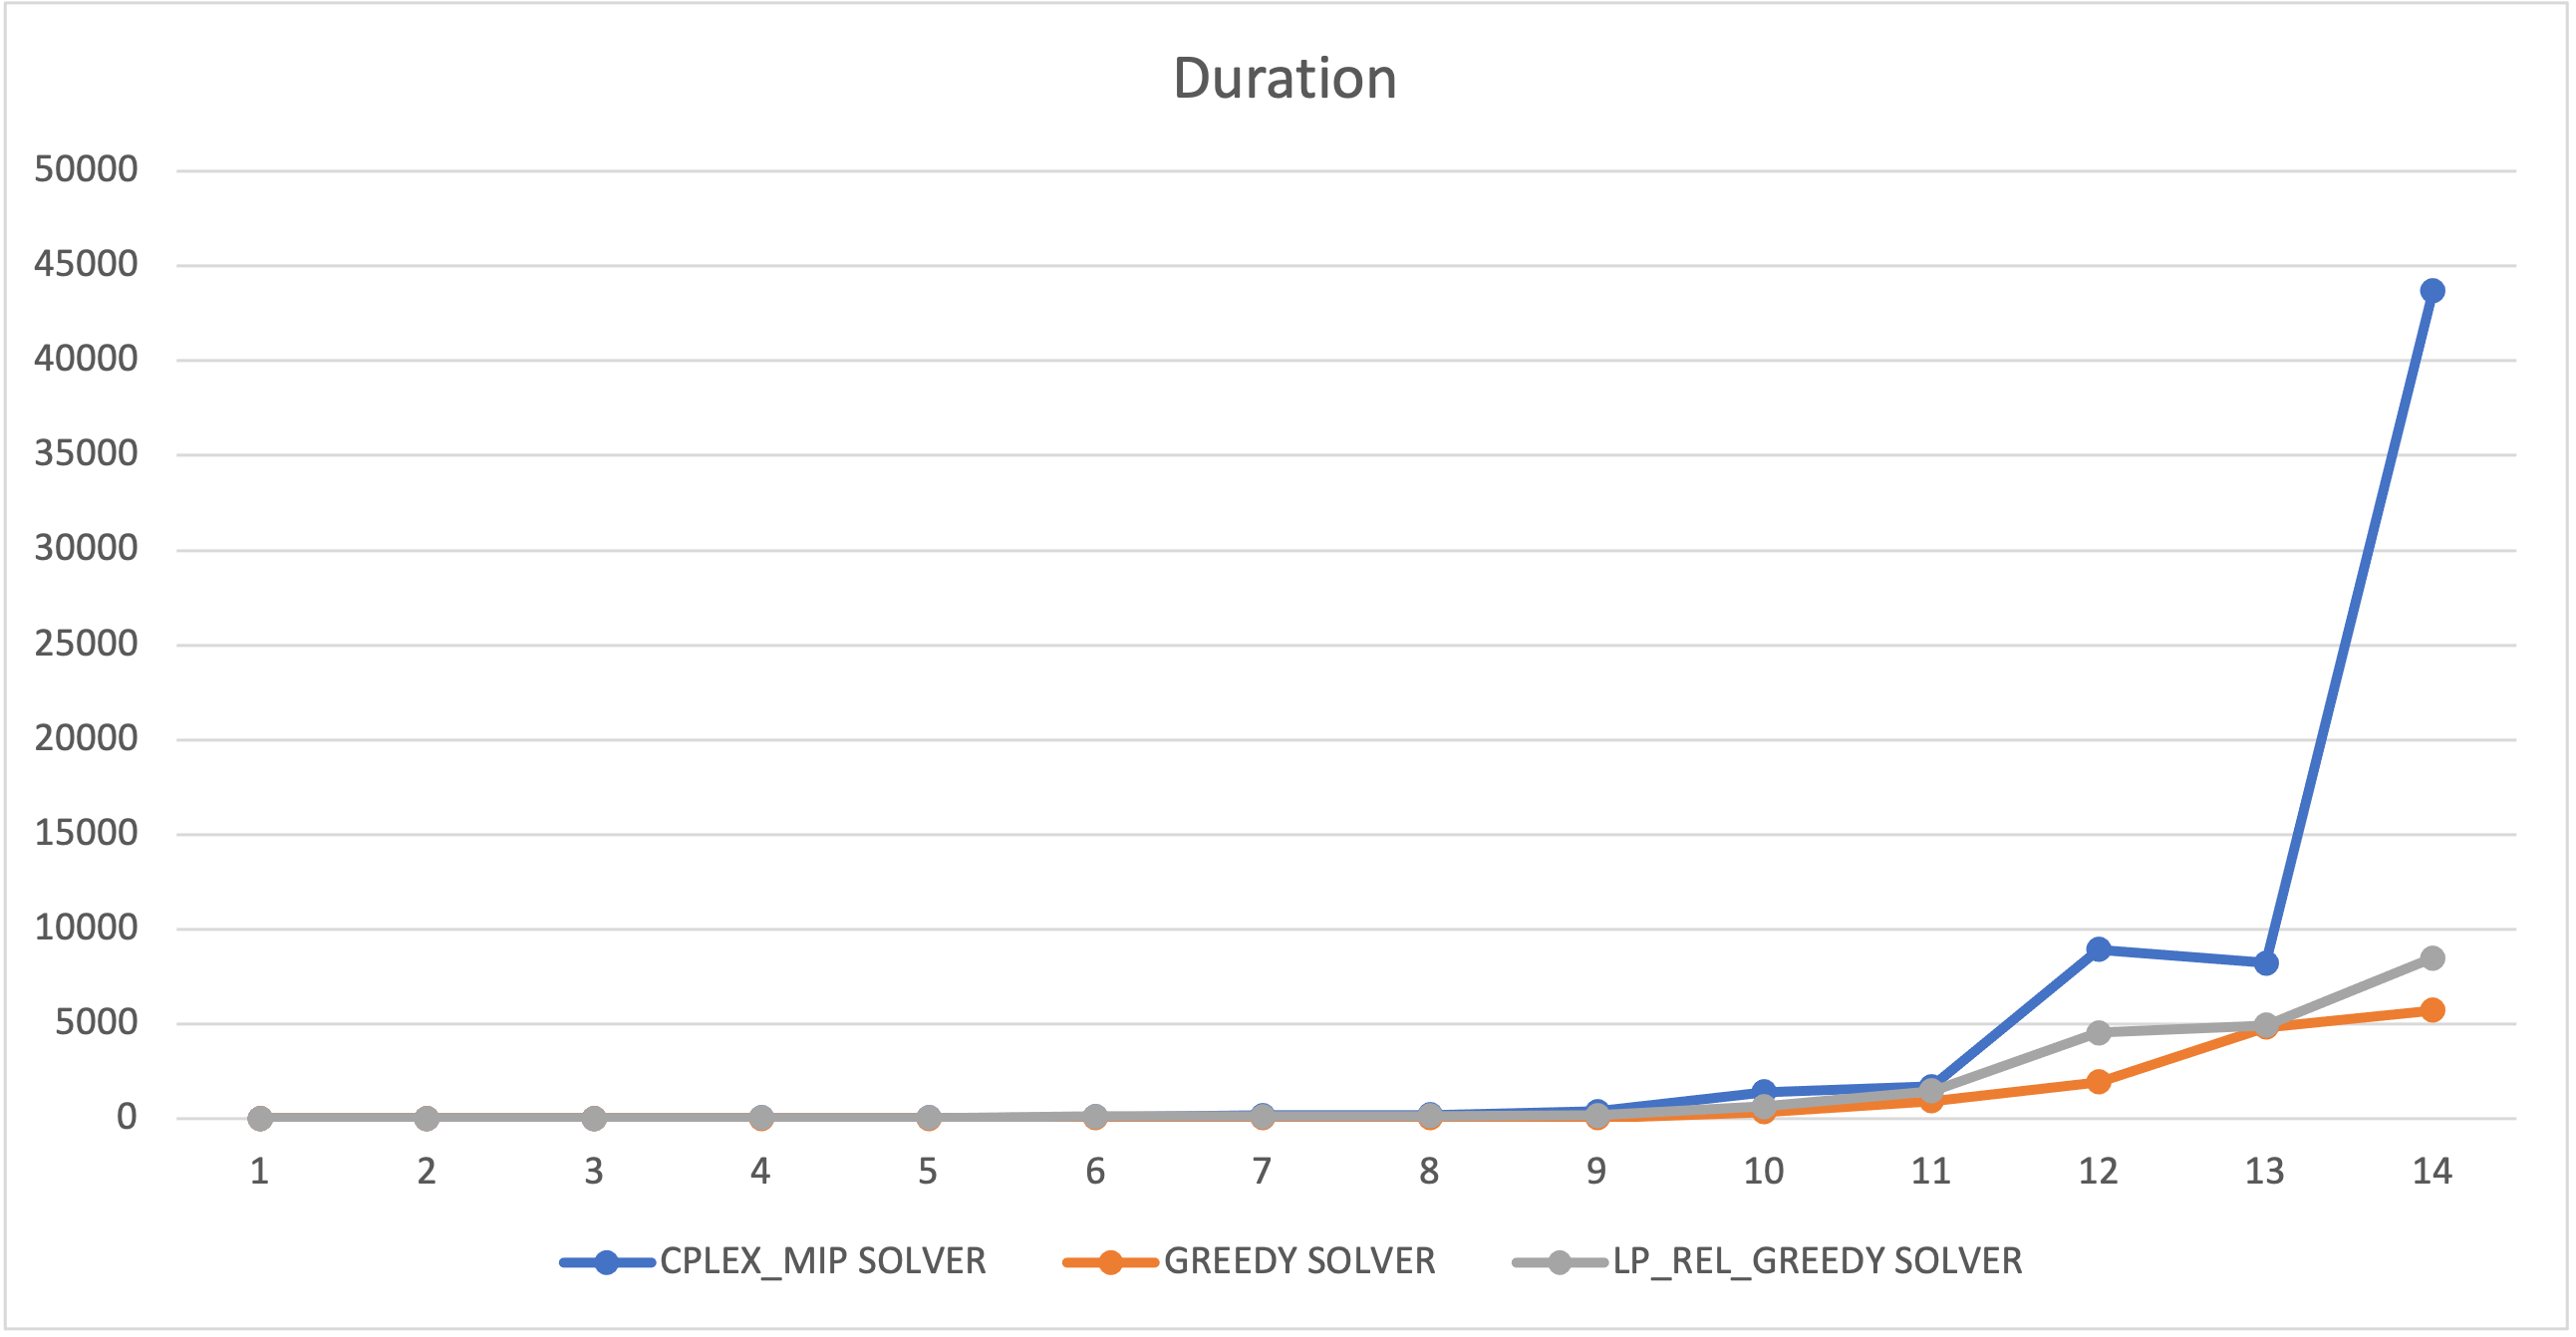
\includegraphics[width=12cm]{durations_no_rh}
            \caption{Durations-No Rolling Horizon Constraints}
            \label{fig:fig_durations_no_rh}
        \end{figure}

        \begin{table}[htb]
                \centering
                \caption[Short Caption for LoT]{\% Objective Value Differentiation-No Rolling Horizon Constraints}\label{table:tbl_test_obj_diff_no_rh}
            \csvautobooktabular{test_results_objective_diff_no_rh.csv}
        \end{table}
        \begin{figure}[htp]
            \centering
            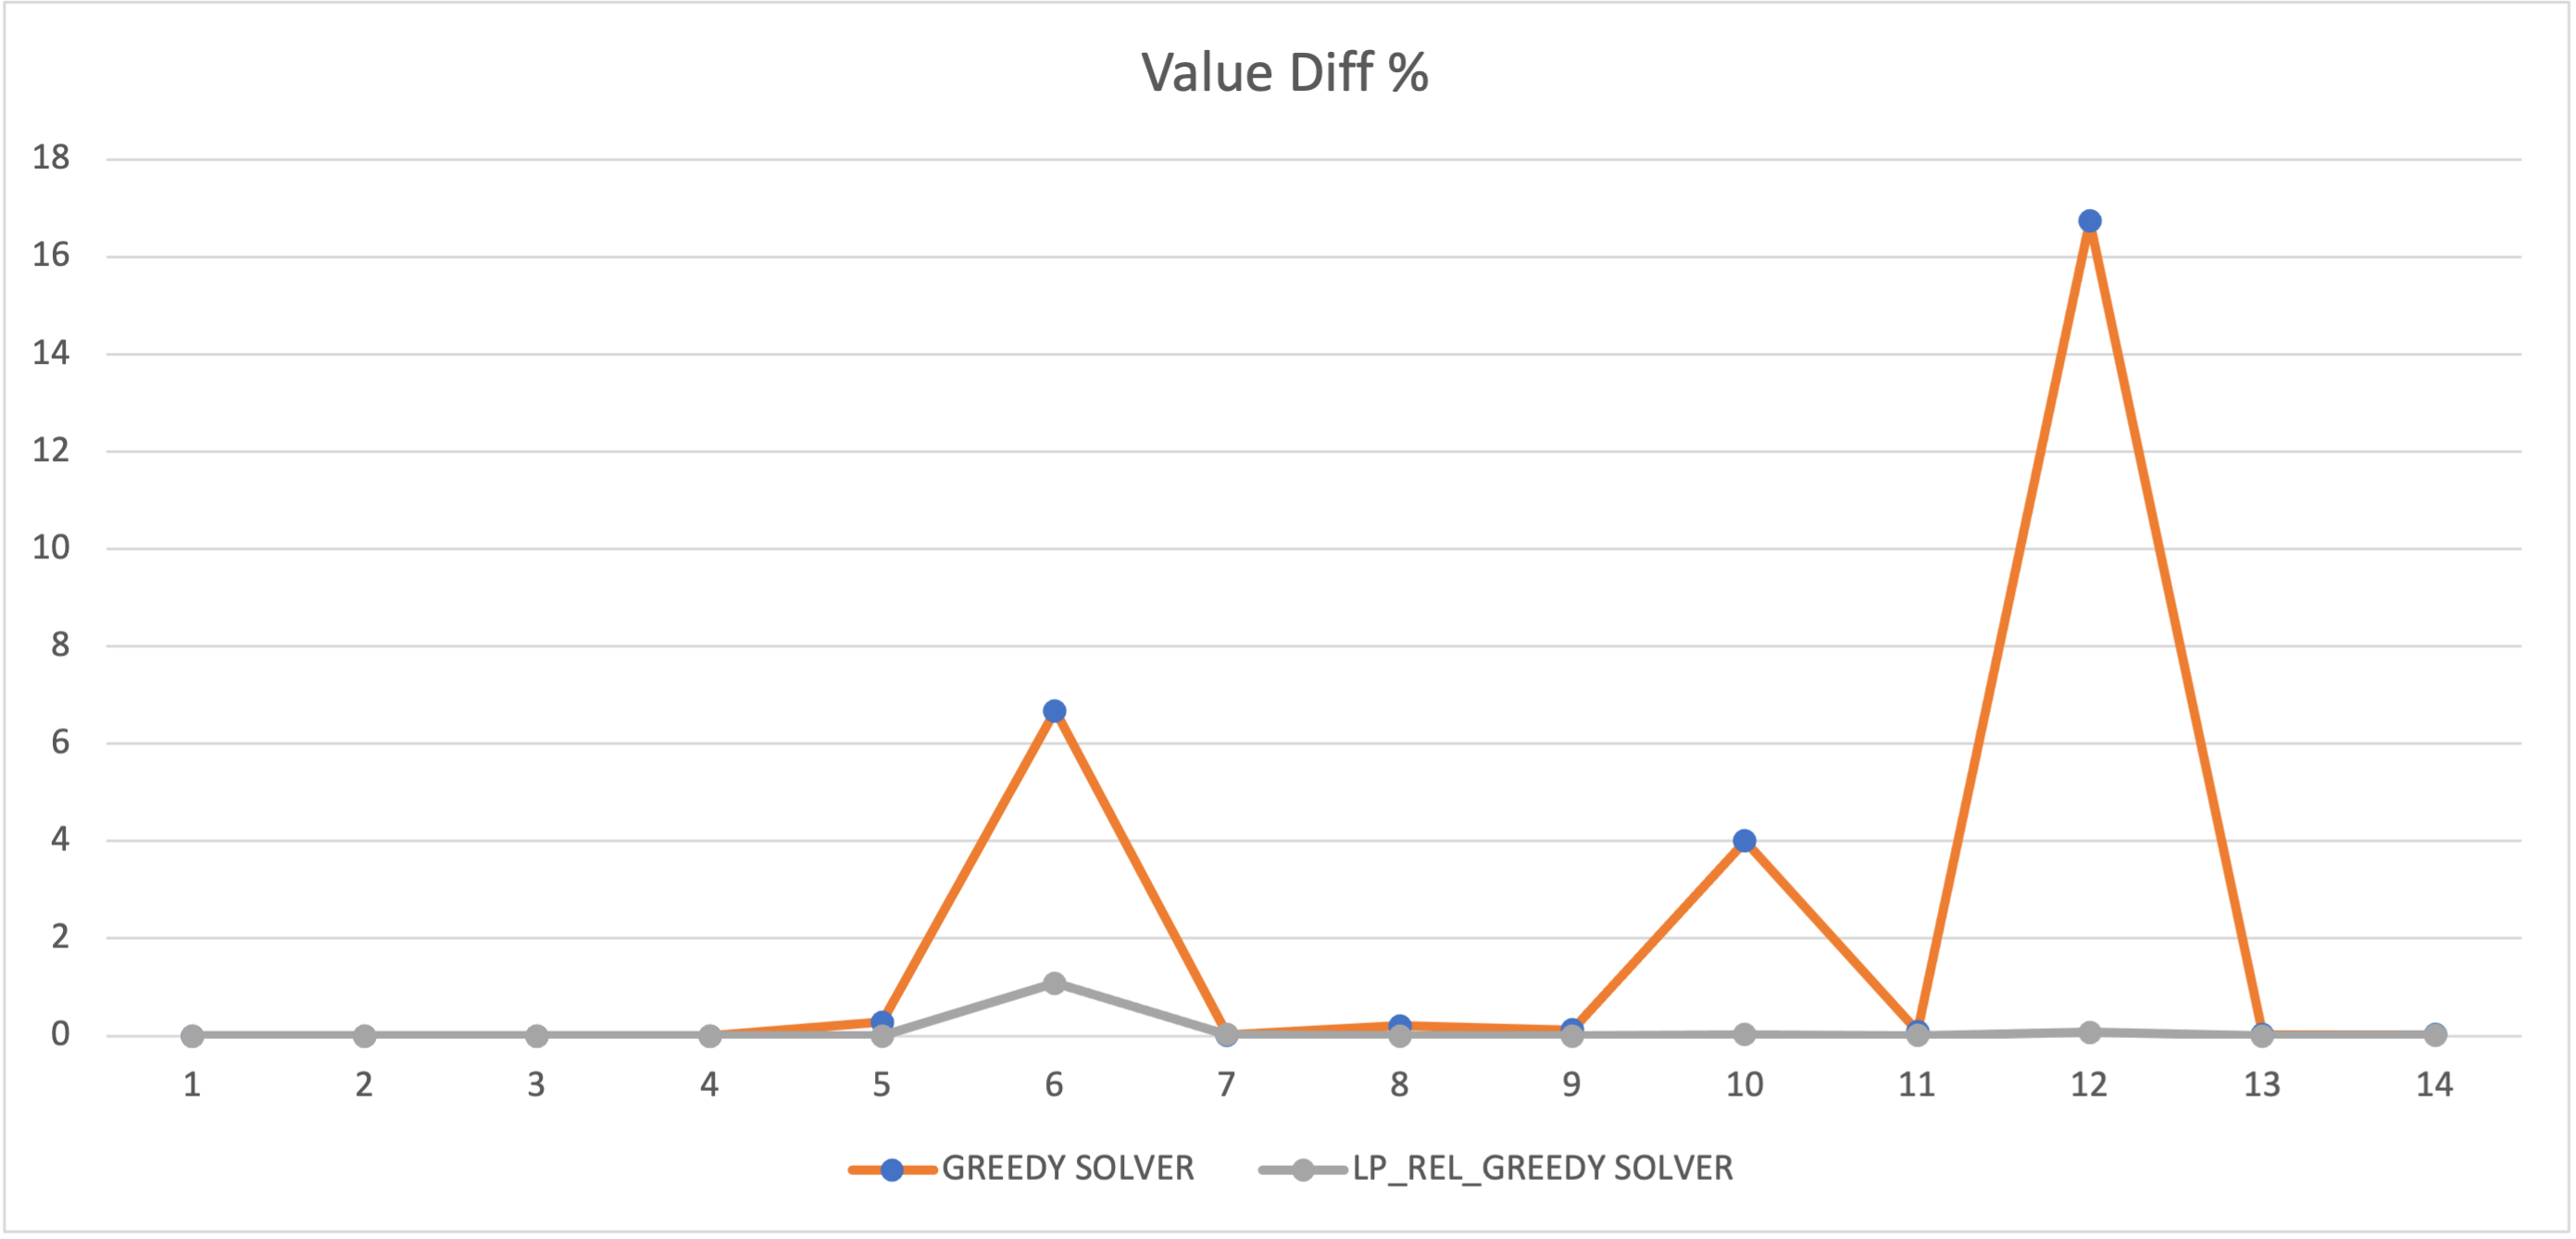
\includegraphics[width=12cm]{value_diff_no_rh}
            \caption{\% Objective Value Differentiation-No Rolling Horizon Constraints}
            \label{fig:fig_value_diff_no_rh}
        \end{figure}
\newpage
        \begin{table}[htb]
                \centering
                \caption[Short Caption for LoT]{Durations at Phase-2 With Rolling Horizon Constraints}\label{table:tbl_test_durations_with_rh_ph2}
            \csvautobooktabular{test_results_durations_with_rh_ph2.csv}
        \end{table}
        
        \begin{figure}[htp]
            \centering
            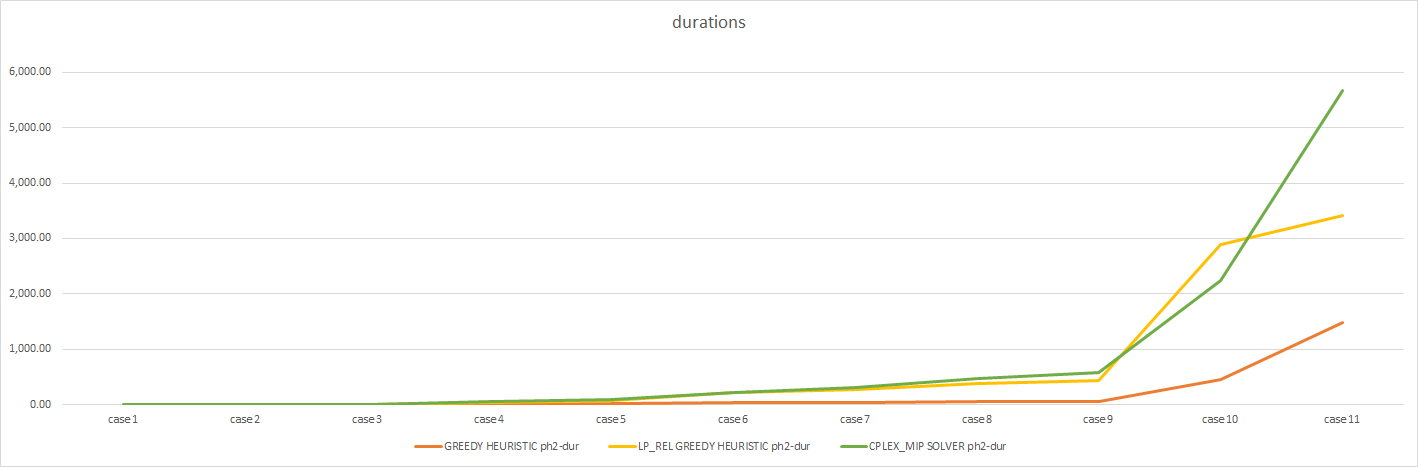
\includegraphics[width=20cm]{durations_with_rh}
            \caption{Durations with Rolling Horizon Constraints}
            \label{fig:fig_durations_with_rh}
        \end{figure}
        
        \begin{table}[htb]
                \centering
                \caption[Short Caption for LoT]{\% Objective Value Differentiation at Phase-2 with Rolling Horizon Constraints}\label{table:tbl_test_obj_diff_with_rh_ph2}
            \csvautobooktabular{test_results_objective_diff_with_rh_ph2.csv}
        \end{table}
        \begin{figure}[htp]
            \centering
            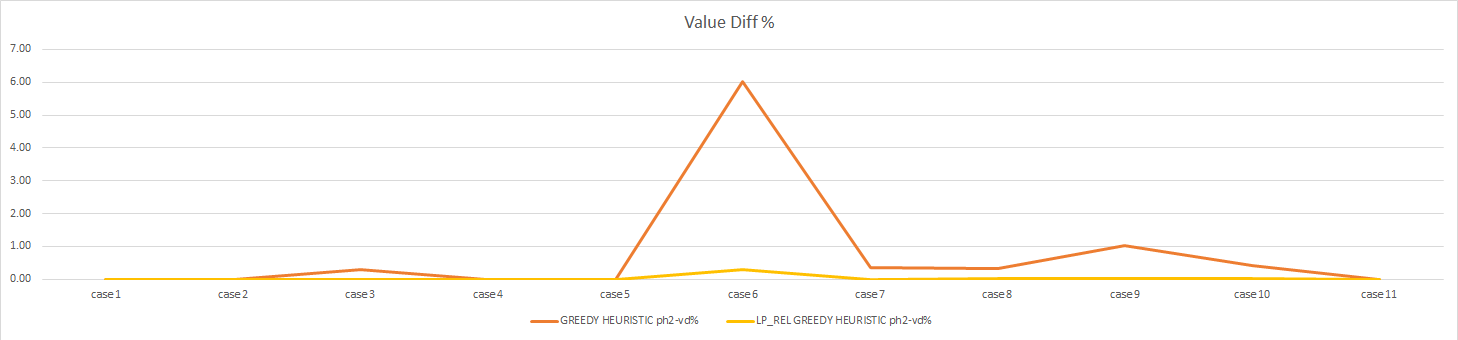
\includegraphics[width=20cm]{value_diff_with_rh}
            \caption{\% Objective Value Differentiation}
            \label{fig:fig_value_diff_with_rh}
        \end{figure}
\newpage
        \begin{table}[htb]
                \centering
                \caption[Short Caption for LoT]{Durations After Betterment-No Rolling Horizon Constraints}\label{table:tbl_test_durations_bett_no_rh}
            \csvautobooktabular{test_results_durations_bett_no_rh.csv}
        \end{table}
        \begin{figure}[htp]
            \centering
            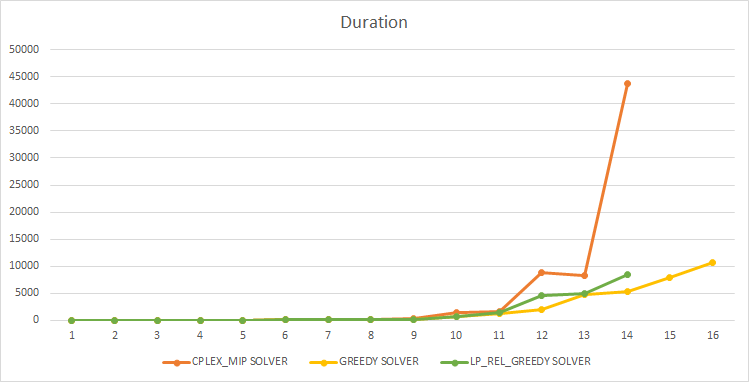
\includegraphics[width=12cm]{durations_bett_no_rh}
            \caption{Durations After Betterment-No Rolling Horizon Constraints}
            \label{fig:fig_durations_bett_no_rh}
        \end{figure}

        \begin{table}[htb]
                \centering
                \caption[Short Caption for LoT]{\% Objective Value Differentiation After Betterment-No Rolling Horizon Constraints}\label{table:tbl_test_obj_diff_bett_no_rh}
            \csvautobooktabular{test_results_objective_diff_bett_no_rh.csv}
        \end{table}
        \begin{figure}[htp]
            \centering
            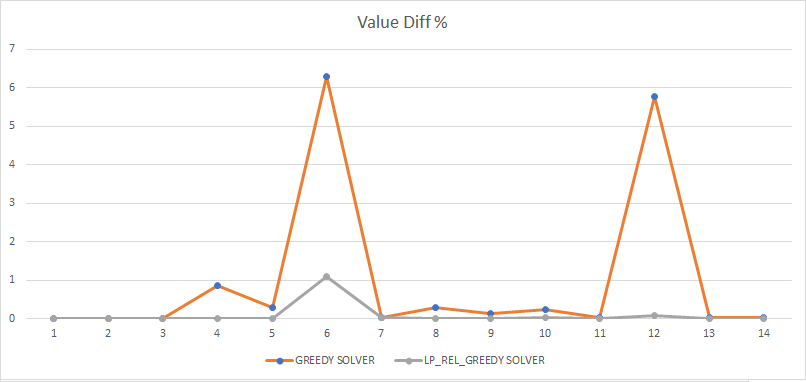
\includegraphics[width=12cm]{value_diff_bett_no_rh}
            \caption{\% Objective Value Differentiation After Betterment-No Rolling Horizon Constraints}
            \label{fig:fig_value_diff_bett_no_rh}
        \end{figure}
    \end{landscape}
    \clearpage% Flush page
}

%%%%%%%%%%%%%%%%%%%%%%%%%%%%%%%%%%%%%%%%%%%%%%%%%%%%%%%%%%
%%%%%%%%%%%%%%%%%%%%%%%%%%%%%%%%%%%%%%%%%%%%%%%%%%%%%%%%%%

\newpage

\section{Conclusion} \label{s:conclusion}
In this study, we discussed a campaign optimization problem, prior to this study literature mostly discussed the problems on finding right target audience, and optimization of it, against cost of delivery and return of investment. In this study our approach is to optimize an existing target audience against communication limitations, both not to irritate customer and be compliant with regulations such as GDPR. We mathematically modeled the problem described at \S \ref{s:problem-math} and later at \S \ref{s:solution-method} offered three heuristic to solve it. A greedy approach that starts with a small LP-model described at \S \ref{s:greedy_heuristic_improved} seems to find good solutions with-in reasonable duration with low memory and cpu.\\
Future research can focus on developing alternative solution methods for the proposed campaign optimization problem. Moreover, proposed problem does not offer a target audience optimization considering the network effect between people. Future research can extend the proposed problem by adding more constraint to cover whole customer network to utilize the communication between people.

\newpage

\bibliographystyle{chicago}
\bibliography{references}

\end{document}